\documentclass[conference]{IEEEtran}
\IEEEoverridecommandlockouts
\usepackage{cite}
\usepackage{amsmath,amssymb}
\usepackage{graphicx}
\usepackage{xcolor}
\usepackage{listings}
\usepackage{url}
\usepackage{booktabs}

\lstdefinestyle{ccode}{
  language=C,
  basicstyle=\ttfamily\scriptsize,
  breaklines=true,
  frame=single,
  numbers=left,
  numberstyle=\tiny\color{gray},
  keywordstyle=\color{blue!70!black},
  commentstyle=\color{green!40!black},
  showstringspaces=false,
  columns=fullflexible
}
\lstdefinestyle{asm}{
  basicstyle=\ttfamily\scriptsize,
  breaklines=true,
  frame=single,
  numbers=none,
  commentstyle=\color{gray},
  showstringspaces=false,
  columns=fullflexible
}

\begin{document}

\title{On the Resistance of Protected Executables to\\
AI-Assisted Reverse Engineering:\\
A Measurement Study}

\author{
\IEEEauthorblockN{Charbel J. Estephan}
\IEEEauthorblockA{Dept.\ of Computer and Communications Engineering\\
Notre Dame University -- Louaize\\
Zouk Mosbeh, Lebanon}
\and
\IEEEauthorblockN{[Second Author]}
\IEEEauthorblockA{Dept.\ of Computer and Communications Engineering\\
Notre Dame University -- Louaize\\
Zouk Mosbeh, Lebanon}
}

\maketitle

\begin{abstract}
Large language models (LLMs) are increasingly used to accelerate reverse
engineering of compiled software, recovering function names, variable names,
and natural-language descriptions directly from stripped binaries. This raises
a practical question for software protection: can an executable be made hard
for an AI system to understand? We argue that ``AI resistance'' is not a new
attack surface but a degradation of the same artifacts a human analyst
consumes, namely symbols, strings, data constants, and recoverable control
flow. We build a small, reproducible testbed of four C programs with known
ground truth, apply three cumulative protection levels (none; symbol stripping
with compiler optimization; manual control-flow flattening with opaque
predicates and string encryption), and measure how much of each program's
purpose and secret an analyst can recover from the resulting binaries. Using an
LLM as the analyst, mean purpose-recovery falls from 5.0/5 at the unprotected
level to 2.0/5 under obfuscation, while mean secret-recovery falls only from
5.0/5 to 3.5/5. A disassembly walkthrough explains the gap: obfuscation turns
linear control flow into an indirect jump table and encrypts strings, yet the
defining data constants and arithmetic survive in the instruction stream. We
conclude that defeating AI-assisted analysis requires techniques that hide data
and semantics, such as binary virtualization, and that any claim of
``inaccessibility'' should be stated as measurable delay, not denial.
\end{abstract}

\begin{IEEEkeywords}
software protection, reverse engineering, code obfuscation, large language
models, binary analysis, anti-tampering, control-flow flattening
\end{IEEEkeywords}

\section{Introduction}
Compiled software ships as machine code, but machine code is not opaque. Decades
of work in reverse engineering (RE) have produced mature disassemblers and
decompilers that reconstruct readable, C-like pseudocode from binaries. More
recently, large language models have been trained specifically to read compiled
code: systems such as LLM4Decompile~\cite{llm4decompile} decompile binaries
end-to-end, and a growing line of work recovers function names, variable names,
and data structures from \emph{stripped} binaries~\cite{resym,gennm,funcname,howfar}.
For a developer who wants to protect intellectual property, a license check, or
a proprietary algorithm, this prompts a direct question: \emph{can I make my
executable hard for an AI to understand?}

This paper takes that question seriously and answers it empirically. Our central
claim is that AI-assisted RE does not introduce a fundamentally new capability;
it automates and scales the consumption of the same artifacts a human analyst
has always relied on: symbol tables, readable strings, embedded data constants,
and a recoverable control-flow graph (CFG). Consequently, making an executable
``AI resistant'' reduces to \emph{degrading those artifacts}. Where AI differs
from a human is in its weaknesses: context-window limits on large functions,
heavy dependence on familiar code idioms and naming, and brittleness in the face
of synthetic or flattened control flow. A protection strategy aimed at AI should
target exactly these weaknesses.

The word ``inaccessible'' deserves early scrutiny. No static protection can make
a program that runs on a CPU permanently unreadable, because the CPU itself must
eventually execute ordinary instructions. Everything we discuss raises the cost
of understanding; none of it reduces that cost to infinity. The useful question
is therefore quantitative: how much does a given protection slow an analyst, and
which artifact does it take away? We adopt that framing throughout.

\textbf{Contributions.} This paper makes the following contributions:
\begin{itemize}
\item We frame AI resistance as artifact degradation and give a threat model
that separates what an AI-assisted analyst can and cannot recover
(Section~\ref{sec:threat}).
\item We catalogue the specific weaknesses of LLM analysts and tie each to a
defensive lever (Section~\ref{sec:weak}).
\item We present a taxonomy of common protections and map each to the artifact
it degrades, with a short treatment of how each works and what it costs
(Section~\ref{sec:taxonomy}).
\item We build a small, fully reproducible testbed and measure recovery across
three cumulative protection levels, reporting static indicators, an LLM-analyst
recovery score, and a disassembly-level walkthrough
(Sections~\ref{sec:method}--\ref{sec:eval}).
\item We identify and quantify a concrete limitation of lightweight,
source-level obfuscation: it hides names, strings, and structure but not data
constants, leaving embedded secrets recoverable, and we translate the finding
into a layered defender's playbook (Section~\ref{sec:discuss}).
\end{itemize}

\section{Background}
\subsection{The Reverse Engineering Pipeline}
Static RE of a native executable proceeds in stages. A loader-aware parser reads
the file format (ELF or PE) and locates sections, imports, and symbols. A
disassembler recovers instructions, which is already non-trivial on variable
length instruction sets such as x86 where code and data interleave. A decompiler
then lifts instructions into an intermediate representation, reconstructs the
control-flow graph, recovers types and variables, and finally structures the CFG
into high-level constructs (loops, conditionals) to emit C-like
pseudocode~\cite{nomoregotos}. Industry tools such as IDA Pro~\cite{idabook} and
Ghidra~\cite{ghidra} implement this pipeline, and binary-analysis frameworks such
as angr~\cite{angr} add symbolic execution and automated reasoning on top.

\subsection{The Four Artifacts}
Throughout the pipeline, the analyst leans on four artifacts, and every
protection in this paper attacks one or more of them:
\begin{enumerate}
\item \textbf{Symbols.} Names of functions and variables. A non-stripped binary
hands the analyst a labelled map; stripping removes it and forces the analyst to
infer roles, the precise task LLM name-recovery tools target~\cite{gennm,funcname}.
\item \textbf{Strings.} Human-readable literals: prompts, error messages, format
strings, URLs, registry paths. Strings are the single most productive triage
signal because they announce intent in natural language.
\item \textbf{Data constants.} Magic numbers, keys, thresholds, and the small
integer arithmetic that defines an algorithm. Constants live inside instructions
(\texttt{cmp \$0x3F7}, \texttt{lea (\%rax,\%rax,2)}) and ordinarily survive every
transformation short of moving the computation off native code.
\item \textbf{Recoverable CFG.} The shape of control flow. When it mirrors the
source, loops and branches read like the original program; destroying it is the
goal of control-flow flattening.
\end{enumerate}

\subsection{AI-Assisted Reverse Engineering}
LLM-based tools consume these same artifacts, usually as disassembly or decompiler
pseudocode. LLM4Decompile reports end-to-end decompilation that improves
re-executability over both GPT-4 and raw Ghidra output~\cite{llm4decompile}.
ReSym recovers variable names and user-defined data structures by combining an
LLM with program analysis~\cite{resym}; GenNm and domain-adapted models recover
names for stripped functions~\cite{gennm,funcname}. Empirical studies measure how
far these models have come on real stripped binaries and find real but uneven
capability, strongly dependent on the presence of recoverable structure and
idioms~\cite{howfar,empirical}. This dependence is the opening a defender
exploits: remove the idioms and the model loses its footing faster than a patient
human does.

\section{Where AI Analysts Are Weak}\label{sec:weak}
A protection aimed at AI should press on the model's weaknesses rather than treat
it as an omniscient oracle. We identify four, each supported by the empirical
literature and each mapped to a defensive lever.

\textbf{Context-window limits.} An LLM reasons over a bounded token window. A
function that is small in source can, after inlining and flattening, expand into
hundreds of instructions that exceed what the model can hold while also keeping
global state in view. A human analyst offloads this to notes and a debugger; the
model does not. \emph{Lever:} inflate function size through flattening and
inlining.

\textbf{Idiom and naming dependence.} Models are trained on ordinary compiler
output and lean heavily on familiar idioms and on symbol names when present;
studies of stripped-binary understanding report sharp drops when these cues are
absent~\cite{howfar,empirical}. \emph{Lever:} strip symbols and replace natural
control flow with synthetic dispatch.

\textbf{Brittleness and confident error.} Faced with opaque predicates and bogus
control flow, models tend to produce fluent but wrong explanations rather than
admit uncertainty, because they are optimized to continue plausibly.
\emph{Lever:} inject dead branches and opaque predicates that look meaningful.

\textbf{Static-only view.} Most LLM analysis is static. Behavior that only
materializes at run time, such as a string decrypted in memory or code unpacked
on demand, is invisible to a purely static reading. \emph{Lever:} defer secrets
to run time through string encryption and packing.

These levers are exactly the techniques in our taxonomy. The study that follows
asks how much each one actually buys.

\section{Threat Model}\label{sec:threat}
We assume an analyst who possesses the protected executable and standard tooling
(a disassembler, a decompiler, and an LLM-based assistant) but not the source
code, debug information, or the build environment. We distinguish two analyst
tiers. A \emph{triage} analyst performs fast, shallow passes: run
\texttt{strings}, skim the symbol table, ask an LLM to summarize a decompiled
function. A \emph{determined} analyst invests time: traces a flattened
dispatcher state by state, recovers constants, and if needed turns to dynamic
analysis. We measure static recovery and treat dynamic analysis as out of scope
for measurement, discussing it as a defense-defeating avenue in
Section~\ref{sec:discuss}.

The analyst's goals are two:
\begin{itemize}
\item \textbf{Purpose recovery:} state what the program does at a functional
level (``it validates a license key''; ``it computes a Collatz stopping time'').
\item \textbf{Secret recovery:} extract the protected value or mechanism (the
accepted key and the check that enforces it; the exact arithmetic of the
algorithm).
\end{itemize}
The defender's goal is to maximize the analyst's time and error rate on both,
subject to preserving program behavior and keeping size and performance overhead
acceptable. We do \emph{not} claim any defender can make recovery impossible; the
metric is how far recovery degrades, and for whom.

\section{Taxonomy of Protections}\label{sec:taxonomy}
Table~\ref{tab:taxonomy} organizes common protections by the artifact each one
attacks. This mapping is the practical core of the paper: it says, for a given
protection, which part of the analyst's input disappears.

\begin{table}[t]
\caption{Protections mapped to the analyst artifact they degrade.}
\label{tab:taxonomy}
\centering
\footnotesize
\begin{tabular}{@{}p{2.3cm}p{2.0cm}p{2.7cm}@{}}
\toprule
\textbf{Technique} & \textbf{Artifact degraded} & \textbf{Effect on AI analyst} \\
\midrule
Symbol stripping & Symbols & Removes names; model must infer them~\cite{gennm,funcname} \\
String encryption & Strings & Removes plaintext intent leaks \\
Control-flow flattening~\cite{obf-taxonomy,ollvm} & Recoverable CFG & Destroys linear flow and idioms \\
Opaque predicates~\cite{obf-taxonomy} & Recoverable CFG & Injects dead edges, confuses structuring \\
Packing / runtime decryption & All (statically) & Hides code until unpacked at run time \\
Code virtualization & CFG + data + semantics & Replaces native code with custom bytecode \\
Anti-debug / anti-VM & Dynamic analysis & Blocks the pipelines that feed AI \\
\bottomrule
\end{tabular}
\end{table}

\subsection{Symbol Stripping}
The cheapest protection removes the symbol table (\texttt{strip -s}), erasing
function and variable names and often the boundaries between functions. It costs
nothing at run time and is reversible only by inference. Against AI it is weak on
its own: optimized code remains linear and idiom-rich, and name recovery is a
solved-enough problem for modern tools~\cite{gennm,funcname,howfar}.

\subsection{String Encryption}
Output and data strings are stored XOR- or cipher-encrypted and decrypted into a
buffer at run time, so no plaintext appears in the static image. The cost is a
small decrypt routine and negligible runtime overhead. The payoff is
disproportionate, because it removes the fastest triage signal entirely: a
\texttt{strings} pass and an LLM summary that keys on messages both come up empty.

\subsection{Control-Flow Flattening}
Flattening rewrites a function's natural control flow into a single dispatcher
loop over an explicit state variable, so the CFG becomes a flat ``switch inside a
while'' with no direct correspondence to the source~\cite{obf-taxonomy,ollvm}.
Compilers frequently lower the dispatcher to an indirect jump through a jump
table, which is exactly what we observe in Section~\ref{sec:eval}. This destroys
the linear structure an analyst (human or model) reads intent from, at a modest
runtime cost.

\subsection{Opaque Predicates}
An opaque predicate is a condition whose truth value is known to the defender at
obfuscation time but is hard to determine statically, for example $x^2-x \equiv 0
\pmod 2$, which is always true. Inserted as a branch guard, it lets the defender
attach plausible-looking dead code that never executes, inflating the CFG and
inviting the analyst to waste effort or hallucinate purpose for the dead path.

\subsection{Packing and Virtualization}
Packers compress or encrypt the whole code section and restore it in memory at
launch, so a static image shows only a stub. Virtualization goes further:
the protected logic is compiled to a custom bytecode executed by an embedded
interpreter, so there is no native instruction implementing the original
operation at all~\cite{protecting-survey}. Virtualization is the only technique
in the table that hides \emph{data and semantics}, not merely structure, and is
correspondingly the most expensive in size and speed.

\subsection{Anti-Debugging and Anti-VM}
These runtime checks detect debuggers, emulators, and sandboxes and alter
behavior when found. They do not hide static content; they attack the
\emph{dynamic} pipeline that an analyst falls back on when static analysis
stalls, and thereby protect the other techniques from being peeled apart at run
time.

Two observations close the taxonomy. First, the techniques are cumulative and
complementary: each removes a different artifact, so strength comes from stacking
them. Second, only virtualization targets data constants and semantics; the
lighter techniques leave embedded values in place. That gap is the study's main
empirical finding.

\section{Methodology}\label{sec:method}
\subsection{Samples and Ground Truth}
We use four small C programs chosen so that their behavior is crisp and
independently checkable, which lets us score recovery objectively. The set spans
the two things developers actually protect, a hidden value and a hidden
algorithm, and spans both arithmetic-heavy and branch-heavy code.
Listing~\ref{lst:p1} and Listing~\ref{lst:p2} give two of the unprotected sources.
\begin{itemize}
\item \textbf{P1 (license validator).} Reads a password, XORs each character with
the constant \texttt{0x5A}, sums the results, and grants access iff the sum
equals \texttt{0x3F7} (1015). It prints \texttt{ACCESS GRANTED} or
\texttt{ACCESS DENIED}. Ground truth: the check logic and the two constants.
\item \textbf{P2 (Collatz stopping time).} Reads an integer $n$ and applies the
Collatz map ($n/2$ if even, $3n+1$ if odd) until $n=1$, printing the number of
steps. Ground truth: the Collatz identity and its branch structure.
\item \textbf{P3 (djb2 hash key check).} Computes the djb2 string hash of the
input (seed \texttt{5381}, multiplier $33$ via \texttt{(h<<5)+h}) and grants iff
it equals a target constant. Ground truth: the djb2 algorithm, its seed, and the
target. This tests recovery of a recognizable named algorithm.
\item \textbf{P4 (serial validator).} Accepts an eight-digit serial whose last
digit is the mod-10 check digit of the first seven. Ground truth: the length and
digit checks and the mod-10 rule. This is deliberately branch-heavy, to stress
control-flow flattening.
\end{itemize}
P1 and P3 protect a secret \emph{value} (a key); P2 and P3 protect a secret
\emph{algorithm}; P4 protects branch-heavy validation \emph{logic}. Together they
let us ask whether the recovery trends hold across code of different shape.

\begin{lstlisting}[style=ccode,caption={P1 license validator (unprotected).},label={lst:p1}]
static int validate(const char *pw) {
    int acc = 0;
    for (size_t i = 0; i < strlen(pw); i++)
        acc += (pw[i] ^ 0x5A);
    return acc == 0x3F7;
}
\end{lstlisting}

\begin{lstlisting}[style=ccode,caption={P2 Collatz stopping time (unprotected).},label={lst:p2}]
static unsigned long collatz_steps(unsigned long n) {
    unsigned long steps = 0;
    while (n != 1) {
        if (n % 2 == 0) n = n / 2;
        else            n = 3 * n + 1;
        steps++;
    }
    return steps;
}
\end{lstlisting}

\subsection{Protection Levels}
We compile three cumulative variants of each program:
\begin{itemize}
\item \textbf{L0 (none):} \texttt{gcc -O0}, symbols retained.
\item \textbf{L1 (strip+opt):} \texttt{gcc -O2} followed by \texttt{strip -s}.
\item \textbf{L2 (obfuscated):} a manually rewritten source applying control-flow
flattening (a dispatcher loop over an explicit state variable), opaque
predicates, and string encryption, then \texttt{gcc -O2} and \texttt{strip -s}.
\end{itemize}
Listing~\ref{lst:flatten} shows the flattening pattern used at L2: the original
linear loop becomes a state machine whose transitions are guarded by an opaque
predicate \texttt{OP}, with an unreachable sink state that never executes because
\texttt{OP} is always true.

\begin{lstlisting}[style=ccode,caption={Control-flow flattening at L2 (P1 validator, abridged).},label={lst:flatten}]
#define OP(x) ((((unsigned)(x)*(unsigned)(x) \
               - (unsigned)(x)) & 1u) == 0u) /* always true */
int state = 0, acc = 0; size_t i = 0;
for (;;) switch (state) {
  case 0: if (OP(len)){acc=0;i=0;state=1;} else state=99; break;
  case 1: state = (i < len) ? 2 : 3; break;
  case 2: acc += (pw[i]^0x5A); i++;
          state = OP(i) ? 1 : 99; break;
  case 3: result = (acc == 0x3F7); state = 100; break;
  case 99: acc ^= 0xFFFF; state = 1; break; /* dead sink */
  case 100: return result;
}
\end{lstlisting}

We verified that all three variants of each program produce identical output on a
battery of inputs, including the valid password and the classic check that the
Collatz stopping time of 27 is 111 steps. Protection that changes behavior is
useless, so this equivalence check is a precondition for the rest of the study.

Because a commercial protector and a dedicated obfuscator (e.g., Tigress,
VMProtect) were not available in our build environment, L2 is a
\emph{source-level} approximation of control-flow flattening. This is a
deliberate, documented limitation: it isolates the effect of flattening,
stripping, and string encryption while keeping the testbed fully reproducible,
and it does not model binary virtualization, whose absence we show to matter.

\subsection{Metrics}
We report two kinds of measurement.
\begin{enumerate}
\item \textbf{Static indicators} extracted directly from each binary: file size,
symbol count (\texttt{nm}), readable string count (\texttt{strings}), and whether
the plaintext secret output string is present. These are objective and scripted.
\item \textbf{Analyst recovery scores} on a 0--5 scale for purpose and for
secret, assigned from a reading of the \texttt{objdump} disassembly of each
variant. A score of 5 means full, correct recovery; 0 means no recovery. The
rubric credits concrete evidence: located constants, identified
loop/parity/halving operations, and a correct functional description.
\end{enumerate}

\subsection{Analyst Protocol and a Validity Caveat}
The analyst in this study is an LLM reading the disassembly of each variant. We
record, per variant, which ground-truth facts are recoverable and assign the
rubric scores accordingly. \emph{Threat to validity:} the same model family that
produced the obfuscated source also served as the analyst, so the analyst is not
fully blind. We therefore treat the scores as indicative rather than definitive
and recommend independent replication with a separate model and with human
analysts as future work. The static indicators, which are script-derived and
model-independent, anchor the subjective scores.

\section{Evaluation}\label{sec:eval}
\subsection{Static Indicators}
Table~\ref{tab:static} reports the static measurements across all four programs.
Symbol stripping at L1 removes every user-visible symbol (32--33 per program).
String encryption at L2 is the only technique that removes the plaintext secret
output: \texttt{strings} finds the decision messages (\texttt{ACCESS GRANTED},
\texttt{VALID KEY}, \texttt{SERIAL OK}, and their negatives) at L0 and L1 but not
at L2. P2 prints only a number and so has no secret string to leak (``n/a'').

\begin{table}[t]
\caption{Static protection indicators per program and level.}
\label{tab:static}
\centering
\footnotesize
\begin{tabular}{@{}llcccc@{}}
\toprule
\textbf{Prog} & \textbf{Level} & \textbf{Symbols} & \textbf{Strings} & \textbf{Secret str.} & \textbf{Size (B)} \\
\midrule
P1 & L0 & 33 & 80 & yes & 16088 \\
P1 & L1 & 0  & 46 & yes & 14472 \\
P1 & L2 & 0  & 52 & no  & 14472 \\
P2 & L0 & 33 & 79 & n/a & 16096 \\
P2 & L1 & 0  & 45 & n/a & 14472 \\
P2 & L2 & 0  & 46 & n/a & 14472 \\
P3 & L0 & 32 & 79 & yes & 16040 \\
P3 & L1 & 0  & 44 & yes & 14472 \\
P3 & L2 & 0  & 47 & no  & 14472 \\
P4 & L0 & 33 & 81 & yes & 16080 \\
P4 & L1 & 0  & 47 & yes & 14472 \\
P4 & L2 & 0  & 53 & no  & 14472 \\
\bottomrule
\end{tabular}
\end{table}

\subsection{Control-Flow Complexity}
Table~\ref{tab:cfg} reports a control-flow complexity proxy: the mean number of
conditional branches, unconditional jumps, and indirect jumps per binary at each
level. Because the libc startup code is identical across levels for a given
program, increases reflect the user code. Flattening at L2 raises every measure,
most visibly the indirect-jump count, which rises because the compiler lowers the
state dispatcher to a jump table. The branch-heavy P4 shows the largest jump,
from 17 to 24 unconditional jumps between L0 and L2. This is the objective,
model-independent signature of the structural damage that drives the purpose-recovery
drop in the next subsection.

\begin{table}[t]
\caption{Control-flow complexity (mean per binary over the four programs).}
\label{tab:cfg}
\centering
\footnotesize
\begin{tabular}{@{}lccc@{}}
\toprule
\textbf{Level} & \textbf{Cond.\ branches} & \textbf{Uncond.\ jumps} & \textbf{Indirect jumps} \\
\midrule
L0 (none)       & 11.3 & 14.5 & 6.8 \\
L1 (strip+opt)  & 12.0 & 11.8 & 6.8 \\
L2 (obfuscated) & 15.0 & 18.0 & 8.0 \\
\bottomrule
\end{tabular}
\end{table}

\subsection{Analyst Recovery}
Table~\ref{tab:recovery} and Fig.~\ref{fig:recovery} report recovery. At L0, both
purpose and secret are fully recovered: symbols name the functions, plaintext
strings announce intent, and the constants \texttt{0x3F7} and \texttt{0x5A} (P1)
and the parity test, right shift, and $3n{+}1$ arithmetic (P2) are plainly
visible. At L1, stripping removes names but \texttt{-O2} produces clean, linear
code in which the algorithm and all constants remain recoverable; purpose drops
slightly (to 4/5) only because the analyst must infer roles without names, while
secret recovery stays at 5/5.

\begin{table}[t]
\caption{Analyst recovery scores (0--5).}
\label{tab:recovery}
\centering
\footnotesize
\begin{tabular}{@{}llcc@{}}
\toprule
\textbf{Program} & \textbf{Level} & \textbf{Purpose} & \textbf{Secret} \\
\midrule
P1 & L0 & 5 & 5 \\
P1 & L1 & 4 & 5 \\
P1 & L2 & 2 & 3 \\
P2 & L0 & 5 & 5 \\
P2 & L1 & 4 & 5 \\
P2 & L2 & 2 & 4 \\
P3 & L0 & 5 & 5 \\
P3 & L1 & 4 & 5 \\
P3 & L2 & 2 & 4 \\
P4 & L0 & 5 & 5 \\
P4 & L1 & 4 & 5 \\
P4 & L2 & 2 & 3 \\
\midrule
\textbf{Mean} & L0 & \textbf{5.0} & \textbf{5.0} \\
\textbf{Mean} & L1 & \textbf{4.0} & \textbf{5.0} \\
\textbf{Mean} & L2 & \textbf{2.0} & \textbf{3.5} \\
\bottomrule
\end{tabular}
\end{table}

\begin{figure}[t]
\centering
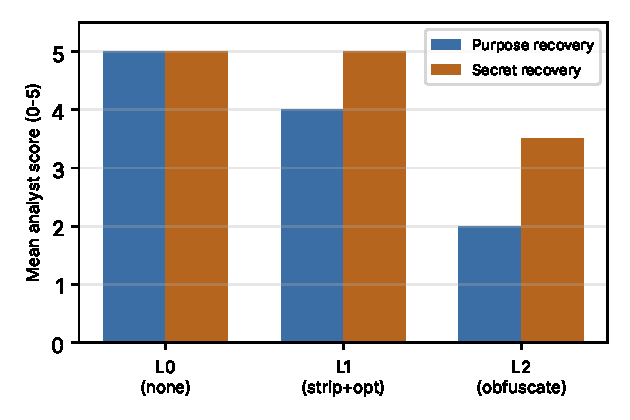
\includegraphics[width=0.80\columnwidth]{recovery.pdf}
\caption{Mean analyst recovery by protection level. Obfuscation sharply reduces
purpose recovery but leaves secret recovery partially intact because data
constants survive source-level transformation.}
\label{fig:recovery}
\end{figure}

\subsection{A Disassembly Walkthrough}
The headline numbers are best understood at the instruction level. Consider P2.
At L0, \texttt{collatz\_steps} disassembles to a short, linear loop
(Listing~\ref{lst:asm-l0}) in which every ground-truth fact is on the surface:
\texttt{and \$0x1} tests parity, \texttt{shr \$1} halves, the sequence
\texttt{add \%rax,\%rax; add \%rdx,\%rax; add \$0x1} computes $2n+n+1=3n+1$, and
\texttt{cmpq \$0x1} is the loop termination. An analyst recovers ``Collatz
stopping time'' in seconds.

\begin{lstlisting}[style=asm,caption={P2 at L0: the Collatz loop is explicit.},label={lst:asm-l0}]
and    $0x1,%eax        ; n & 1  (parity test)
test   %rax,%rax
jne    .odd
shr    $1,%rax          ; n = n / 2
jmp    .next
.odd:
mov    %rdx,%rax
add    %rax,%rax        ; 2n
add    %rdx,%rax        ; 2n + n = 3n
add    $0x1,%rax        ; 3n + 1
.next:
addq   $0x1,-0x8(%rbp)  ; steps++
cmpq   $0x1,-0x18(%rbp) ; while (n != 1)
jne    .loop
\end{lstlisting}

At L2 the picture changes (Listing~\ref{lst:asm-l2}). The compiler lowered the
flattened dispatcher to an \emph{indirect jump through a jump table}
(\texttt{notrack jmp *\%rsi}), so there is no longer a linear loop to read; the
state variable is compared against bounds (\texttt{cmp \$0x9}) and control scatters
across cases. The opaque-predicate dead sink is visible as the never-taken
\texttt{add \$0xdead,\%rdx}. Function boundaries are gone (everything folds into
\texttt{.text}). This is why purpose recovery collapses: the structure that
spelled out ``loop that maps $n$ until 1'' is gone.

\begin{lstlisting}[style=asm,caption={P2 at L2: flattening becomes an indirect jump table, but the arithmetic survives.},label={lst:asm-l2}]
cmp    $0x9,%ecx          ; dispatch on state (bounds check)
...
lea    (%rax,%rax,2),%rax ; 3*n  <-- 3n+1 arithmetic SURVIVES
add    $0x1,%rax          ; +1
...
add    $0xdead,%rdx       ; opaque-predicate dead sink (never run)
...
notrack jmp *%rsi         ; flattened dispatcher (indirect jump)
\end{lstlisting}

Crucially, \texttt{lea (\%rax,\%rax,2)} followed by \texttt{add \$0x1} still
implements $3n+1$ in plain sight, and in P1 the constants \texttt{0x3F7} and
\texttt{0x5A} remain embedded in \texttt{cmp}/\texttt{xor} instructions. A
determined analyst who walks the dispatcher state by state therefore still
reconstructs the secret, which is why secret recovery at L2 falls only to 3.5/5
rather than to zero.

\subsection{Interpretation}
Three results stand out. First, \emph{symbol stripping alone is weak against
capable analysis}: optimized, stripped code is still linear and idiom-rich, and
recovering names is exactly the task modern LLM tools are getting good
at~\cite{gennm,funcname,howfar}. Second, \emph{string encryption delivers
disproportionate value} for its low cost, because it removes the single most
productive triage signal. Third, and most important, \emph{lightweight
obfuscation hides structure but not data}. The purpose/secret gap at L2 is the
measurable signature of this: you can stop an analyst from quickly seeing
\emph{what} the program is while still leaking the exact value that makes it
work.

A secondary observation concerns the two analyst tiers. String encryption and
flattening are highly effective against the \emph{triage} analyst, who relies on
fast signals and gives up when they vanish. They are far less effective against
the \emph{determined} analyst, for whom surviving constants are enough. Protection
choice should therefore follow the threat: triage-grade protection is cheap and
adequate against casual AI summarization, but protecting a genuine secret from a
motivated analyst requires hiding the data plane.

\section{Discussion and Limitations}\label{sec:discuss}
\subsection{Why Constants Survive, and What Fixes It}
Source-level flattening and opaque predicates rearrange control flow; they do not
transform the data plane. The compiler still emits the literal \texttt{0x3F7} into
a \texttt{cmp} instruction and $3n+1$ into an \texttt{lea}. Hiding these requires
moving the computation off native instructions, which is what \emph{code
virtualization} does: the real logic is compiled to a custom bytecode executed by
an embedded interpreter, so there is no native \texttt{cmp 0x3F7} to
find~\cite{protecting-survey}. Commercial protectors (VMProtect, Themida) and
research obfuscators (Tigress, OLLVM~\cite{ollvm}) implement this. Our results
motivate virtualization specifically as the step that closes the purpose/secret
gap, and quantifying that closure is the natural next experiment. A cheaper
intermediate step is packing: our repository includes an optional packing level
(L3, via UPX) that compresses and encrypts the whole code section so a static
image shows only a stub. Packing defeats all static recovery until the program is
unpacked at run time, but unlike virtualization it is trivially reversed by a
dynamic dump, which is why we treat it as a triage-grade layer rather than a
secret-hiding one.

\subsection{A Layered Defender's Playbook}
The measurements suggest a cost-ordered strategy:
\begin{enumerate}
\item \textbf{Always:} strip symbols and encrypt strings. Together they defeat
triage-grade AI analysis at near-zero cost and remove the fastest signals.
\item \textbf{For structure:} apply control-flow flattening and opaque predicates
to the sensitive functions to collapse purpose recovery.
\item \textbf{For secrets:} virtualize the routines that embed keys, thresholds,
or proprietary arithmetic, because only virtualization hides the surviving
constants.
\item \textbf{To protect the above:} add anti-debug and anti-VM checks so the
dynamic pipeline cannot simply peel the layers at run time.
\end{enumerate}
Each layer targets a distinct artifact, and the cost rises with the layer, so a
defender matches depth to the value of what is protected.

\subsection{Protections Are Delay, Not Denial}
Every technique here can be attacked. Packers are unpacked by running the program
and dumping memory; opaque predicates are simplified by symbolic execution and
automated deobfuscation~\cite{angr,udupa}; anti-debug checks are patched out;
even virtualization is defeated by recovering the interpreter and lifting the
bytecode~\cite{rolles}. The honest figure of merit is analyst time, and a rigorous
version of this study would report minutes-to-recovery for human analysts across
levels rather than a 0--5 rubric.

\subsection{Threats to Validity}
Beyond the author/analyst coupling noted in Section~\ref{sec:method}, our testbed
is small (four programs), the obfuscation is source-level rather than a production
protector, and the analyst performs only static analysis. These choices favor
reproducibility and isolation of effects over external validity; the trends we
report (stripping weak, encryption cheap and effective, structure hidden but data
exposed) are consistent with the broader literature~\cite{protecting-survey,
obf-taxonomy} but should be confirmed at larger scale, with production protectors,
with multiple independent models, and with dynamic analysis in scope.

\section{Related Work}
Obfuscation has a long theoretical and practical history. Collberg et al.\
introduced the canonical taxonomy of obfuscating
transformations~\cite{obf-taxonomy} and later framed obfuscation, watermarking,
and tamper-proofing as a unified protection problem~\cite{collberg-tse}; their
book consolidates the area~\cite{surreptitious}. Linn and Debray showed how to
obstruct static disassembly directly~\cite{linn-debray}, and Wang et al.\ studied
obstructing static analysis through control-flow
transformation~\cite{wang-tamper}. Obfuscator-LLVM brought production-grade
obfuscation, including control-flow flattening and bogus control flow, to a
mainstream compiler~\cite{ollvm}; Banescu and Pretschner give a modern
tutorial~\cite{banescu}, and recent surveys consolidate the
field~\cite{protecting-survey}. On the analysis side, Udupa et al.\ studied
automated deobfuscation~\cite{udupa}, Rolles analyzed unpacking of
virtualization obfuscators~\cite{rolles}, Yakdan et al.\ advanced
pattern-independent decompilation~\cite{nomoregotos}, and angr systematized
automated binary analysis~\cite{angr}. The newest and most relevant thread is
AI-assisted RE: LLM4Decompile decompiles end-to-end~\cite{llm4decompile};
ReSym~\cite{resym}, GenNm~\cite{gennm}, and domain-adapted models~\cite{funcname}
recover symbols from stripped binaries; and empirical studies chart how capable
these models are in realistic settings~\cite{howfar,empirical}. Our work sits
between these threads, asking what the protection taxonomy looks like when the
analyst is an LLM and measuring where current lightweight protections succeed and
fail.

\section{Conclusion}
Making an executable ``inaccessible to AI'' is the wrong framing; making it
expensive to understand is the right one. AI-assisted reverse engineering
consumes the same artifacts a human does, so protection is artifact degradation,
and its strength is measurable delay. Our small study shows a clear ordering:
symbol stripping is weak on its own, string encryption is cheap and effective at
blocking triage, and control-flow flattening sharply reduces an analyst's ability
to state a program's purpose, collapsing mean purpose recovery from 5.0 to 2.0 out
of 5. But it also exposes the limit of lightweight protection: constants survive,
so secrets leak even when structure is hidden, and mean secret recovery falls only
to 3.5. Closing that gap requires hiding the data plane, which points to binary
virtualization as the necessary next layer and as the next measurement target.

\section*{Reproducibility}
The four programs, all build commands, the three protection variants, the
disassembly, the figure, and the scripts that compute every number in
Tables~\ref{tab:static}, \ref{tab:cfg}, and~\ref{tab:recovery} are included in the
project repository so that all results can be regenerated from source. The
repository also ships an optional \texttt{pack.sh} that adds a packing level
(L3) with UPX on any machine where the packer is installed, so the packing row
of future work can be reproduced locally.

\begin{thebibliography}{00}
\bibitem{llm4decompile} H.~Tan, Q.~Luo, J.~Li, and Y.~Zhang, ``LLM4Decompile: Decompiling binary code with large language models,'' in \emph{Proc. EMNLP}, 2024. arXiv:2403.05286.
\bibitem{resym} D.~Xie, Z.~Zhang, N.~Jiang, X.~Xu, L.~Tan, and X.~Zhang, ``ReSym: Harnessing LLMs to recover variable and data structure symbols from stripped binaries,'' in \emph{Proc. ACM CCS}, 2024.
\bibitem{gennm} X.~Xu \emph{et al.}, ``Leveraging generative models to recover variable names from stripped binary,'' arXiv:2306.02546, 2024.
\bibitem{funcname} L.~Jiang, X.~Jin, and Z.~Lin, ``Beyond classification: Inferring function names in stripped binaries via domain adapted LLMs,'' in \emph{Proc. NDSS}, 2025.
\bibitem{howfar} X.~Shang \emph{et al.}, ``How far have we gone in stripped binary code understanding using large language models,'' arXiv:2404.09836, 2024.
\bibitem{empirical} X.~Shang, S.~Cheng, G.~Chen \emph{et al.}, ``An empirical study on the effectiveness of large language models for binary code understanding,'' arXiv:2504.21803, 2025.
\bibitem{obf-taxonomy} C.~Collberg, C.~Thomborson, and D.~Low, ``A taxonomy of obfuscating transformations,'' Dept.\ Computer Science, Univ.\ Auckland, Tech.\ Rep.\ 148, 1997.
\bibitem{collberg-tse} C.~Collberg and C.~Thomborson, ``Watermarking, tamper-proofing, and obfuscation: Tools for software protection,'' \emph{IEEE Trans.\ Softw.\ Eng.}, vol.~28, no.~8, pp.~735--746, 2002.
\bibitem{surreptitious} C.~Collberg and J.~Nagra, \emph{Surreptitious Software: Obfuscation, Watermarking, and Tamperproofing for Software Protection}. Addison-Wesley, 2009.
\bibitem{linn-debray} C.~Linn and S.~Debray, ``Obfuscation of executable code to improve resistance to static disassembly,'' in \emph{Proc. ACM CCS}, 2003, pp.~290--299.
\bibitem{wang-tamper} C.~Wang, J.~Hill, J.~Knight, and J.~Davidson, ``Software tamper resistance: Obstructing static analysis of programs,'' Univ.\ Virginia, Tech.\ Rep.\ CS-2000-12, 2000.
\bibitem{ollvm} P.~Junod, J.~Rinaldini, J.~Wehrli, and J.~Michielin, ``Obfuscator-LLVM: Software protection for the masses,'' in \emph{Proc. IEEE/ACM SPRO}, 2015, pp.~3--9.
\bibitem{banescu} S.~Banescu and A.~Pretschner, ``A tutorial on software obfuscation,'' \emph{Advances in Computers}, vol.~108, pp.~283--353, 2018.
\bibitem{protecting-survey} S.~Schrittwieser, S.~Katzenbeisser, J.~Kinder, G.~Merzdovnik, and E.~Weippl, ``Protecting software through obfuscation: Can it keep pace with progress in code analysis?'' \emph{ACM Computing Surveys}, vol.~49, no.~1, 2016.
\bibitem{udupa} S.~Udupa, S.~Debray, and M.~Madou, ``Deobfuscation: Reverse engineering obfuscated code,'' in \emph{Proc. Working Conf.\ Reverse Engineering (WCRE)}, 2005.
\bibitem{rolles} R.~Rolles, ``Unpacking virtualization obfuscators,'' in \emph{Proc. USENIX WOOT}, 2009.
\bibitem{nomoregotos} K.~Yakdan, S.~Eschweiler, E.~Gerhards-Padilla, and M.~Smith, ``No more gotos: Decompilation using pattern-independent control-flow structuring and semantics-preserving transformations,'' in \emph{Proc. NDSS}, 2015.
\bibitem{angr} Y.~Shoshitaishvili \emph{et al.}, ``SoK: (State of) the art of war: Offensive techniques in binary analysis,'' in \emph{Proc. IEEE Symp.\ Security and Privacy}, 2016, pp.~138--157.
\bibitem{ghidra} National Security Agency, ``Ghidra software reverse engineering framework,'' \url{https://ghidra-sre.org}, 2019.
\bibitem{idabook} C.~Eagle, \emph{The IDA Pro Book}, 2nd~ed. No Starch Press, 2011.
\end{thebibliography}

\end{document}
